% XCircuit output "bandpass.tex" for LaTeX input from bandpass.ps
\def\putbox#1#2#3#4{\makebox[0in][l]{\makebox[#1][l]{}\raisebox{\baselineskip}[0in][0in]{\raisebox{#2}[0in][0in]{\scalebox{#3}{#4}}}}}
\def\rightbox#1{\makebox[0in][r]{#1}}
\def\centbox#1{\makebox[0in]{#1}}
\def\topbox#1{\raisebox{-0.60\baselineskip}[0in][0in]{#1}}
\def\midbox#1{\raisebox{-0.20\baselineskip}[0in][0in]{#1}}
   \scalebox{1}{
   \normalsize
   \parbox{6.28646in}{
   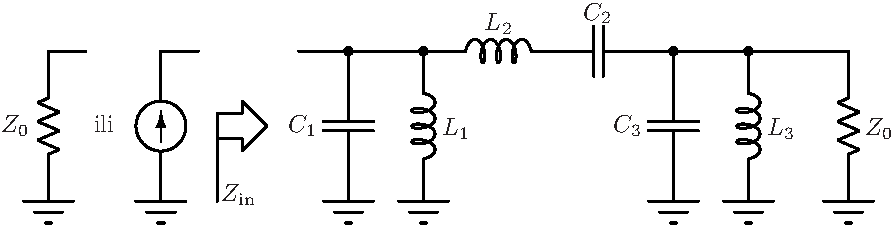
\includegraphics[scale=1]{bandpass}\\
   % translate x=905 y=620 scale 0.38
   \putbox{1.80in}{0.73in}{1.20}{}%
   \putbox{3.14in}{0.64in}{1.20}{$L_1$}%
   \putbox{3.52in}{1.34in}{1.20}{\centbox{$L_2$}}%
   \putbox{4.18in}{1.41in}{1.20}{\centbox{$C_2$}}%
   \putbox{2.31in}{0.70in}{1.20}{\rightbox{\midbox{$C_1$}}}%
   \putbox{4.48in}{0.70in}{1.20}{\rightbox{\midbox{$C_3$}}}%
   \putbox{5.31in}{0.64in}{1.20}{$L_3$}%
   \putbox{5.96in}{0.64in}{1.20}{$Z_0$}%
   \putbox{1.80in}{0.73in}{1.20}{}%
   \putbox{0.39in}{0.70in}{1.20}{\rightbox{\midbox{$Z_0$}}}%
   \putbox{1.67in}{0.20in}{1.20}{\rotatebox{-360}{$Z_\mr{in}$}}%
   \putbox{0.89in}{0.70in}{1.20}{\centbox{\midbox{$\mr{ili}$}}}%
   } % close 'parbox'
   } % close 'scalebox'
   \vspace{-\baselineskip} % this is not necessary, but looks better
